% A LaTeX template for MSc Thesis submissions to 
% Politecnico di Milano (PoliMi) - School of Industrial and Information Engineering
%
% S. Bonetti, A. Gruttadauria, G. Mescolini, A. Zingaro
% e-mail: template-tesi-ingind@polimi.it
%
% Last Revision: October 2021
%
% Copyright 2021 Politecnico di Milano, Italy. NC-BY

\documentclass{config/PoliMi3i_thesis}

%------------------------------------------------------------------------------
%	REQUIRED PACKAGES AND  CONFIGURATIONS
%------------------------------------------------------------------------------

% Uncomment to show margins
%\usepackage{showframe}

% PACKAGE FOR CUSTOM LISTS
\usepackage{enumitem}

% CONFIGURATIONS
\usepackage{parskip} % For paragraph layout
\usepackage{setspace} % For using single or double spacing
\usepackage{emptypage} % To insert empty pages
\usepackage{multicol} % To write in multiple columns (executive summary)
\setlength\columnsep{15pt} % Column separation in executive summary
\setlength\parindent{0pt} % Indentation
\raggedbottom

% PACKAGES FOR TITLES
\usepackage{titlesec}
% \titlespacing{\section}{left spacing}{before spacing}{after spacing}
\titlespacing{\chapter}{0pt}{0ex}{8ex}
\titlespacing{\section}{0pt}{3.3ex}{2ex}
\titlespacing{\subsection}{0pt}{3.3ex}{1.65ex}
\titlespacing{\subsubsection}{0pt}{3.3ex}{1ex}
\usepackage{color}

% PACKAGES FOR LANGUAGE AND FONT
\usepackage[english]{babel} % The document is in English  
\usepackage[utf8]{inputenc} % UTF8 encoding
\usepackage[T1]{fontenc} % Font encoding
\usepackage[11pt]{moresize} % Big fonts

% PACKAGES FOR IMAGES
\usepackage{graphicx}
\usepackage{transparent} % Enables transparent images
\usepackage{eso-pic} % For the background picture on the title page
\usepackage{subfig} % Numbered and caption subfigures using \subfloat.
\usepackage{tikz} % A package for high-quality hand-made figures.
\usetikzlibrary{}
\graphicspath{{./images/}} % Directory of the images
\usepackage{caption} % Coloured captions
\usepackage{xcolor} % Coloured captions
\usepackage{amsthm,thmtools,xcolor} % Coloured "Theorem"
\usepackage{float}
\ifdefined\emitpumldiagrams{}
    \usepackage{svg} % svgs
    \pdfsuppresswarningpagegroup=1 % disable svg export warnings
\fi
\usepackage{adjustbox} % adjust svg size to fit
 
% STANDARD MATH PACKAGES
\usepackage{amsmath}
\usepackage{amsthm}
\usepackage{amssymb}
\usepackage{amsfonts}
\usepackage{bm}
\usepackage[overload]{empheq} % For braced-style systems of equations.
\usepackage{fix-cm} % To override original LaTeX restrictions on sizes

% PACKAGES FOR TABLES
\usepackage{tabularx}
\usepackage{longtable} % Tables that can span several pages
\usepackage{colortbl}
\usepackage{multirow}
\setlength\LTpost{-3.5em}

% PACKAGES FOR ALGORITHMS (PSEUDO-CODE)
\usepackage{algorithm}
\usepackage{algorithmic}
\usepackage{listings}

% PACKAGES FOR REFERENCES & BIBLIOGRAPHY
\PassOptionsToPackage{hyphens}{url}
\usepackage[colorlinks=true,linkcolor=black,anchorcolor=black,citecolor=black,filecolor=black,menucolor=black,runcolor=black,urlcolor=black]{hyperref} % Adds clickable links at references
\usepackage[square, numbers, sort&compress]{natbib} % Square brackets, citing references with numbers, citations sorted by appearance in the text and compressed
\bibliographystyle{abbrvnat} % You may use a different style adapted to your field

% OTHER PACKAGES
\usepackage{pdfpages} % To include a pdf file
\usepackage{afterpage}
\usepackage{lipsum} % DUMMY PACKAGE
\usepackage{fancyhdr} % For the headers
\usepackage{tabu}
\usepackage[]{underscore} % To be able to use _ in text
\fancyhf{}

% Input of configuration file. Do not change config.tex file unless you really know what you are doing. 
% !TeX root = ../rasd.tex
% Define blue color typical of polimi
\definecolor{bluepoli}{cmyk}{0.4,0.1,0,0.4}

% Custom theorem environments
\declaretheoremstyle[
  headfont=\color{bluepoli}\normalfont\bfseries,
  bodyfont=\color{black}\normalfont\itshape,
]{colored}

% Set-up caption colors
\captionsetup[figure]{labelfont={color=bluepoli}} % Set colour of the captions
\captionsetup[table]{labelfont={color=bluepoli}} % Set colour of the captions
\captionsetup[algorithm]{labelfont={color=bluepoli}} % Set colour of the captions

\theoremstyle{colored}
\newtheorem{theorem}{Theorem}[chapter]
\newtheorem{proposition}{Proposition}[chapter]

% Enhances the features of the standard "table" and "tabular" environments.
\newcommand\T{\rule{0pt}{2.6ex}}
\newcommand\B{\rule[-1.2ex]{0pt}{0pt}}

% Pseudo-code algorithm descriptions.
\newcounter{algsubstate}
\renewcommand{\thealgsubstate}{\alph{algsubstate}}
\newenvironment{algsubstates}
{\setcounter{algsubstate}{0}%
  \renewcommand{\STATE}{%
    \stepcounter{algsubstate}%
    \Statex {\small\thealgsubstate:}\space}}
{}

% New font size
\newcommand\numfontsize{\@setfontsize\Huge{200}{60}}

% Title format: chapter
\titleformat{\chapter}[hang]{
  \fontsize{50}{20}\selectfont\bfseries\filright}{\textcolor{bluepoli} \thechapter\hsp\hspace{2mm}\textcolor{bluepoli}{|   }\hsp}{0pt}{\huge\bfseries \textcolor{bluepoli}
}

% Title format: section
\titleformat{\section}
{\color{bluepoli}\normalfont\Large\bfseries}
{\color{bluepoli}\thesection.}{1em}{}

% Title format: subsection
\titleformat{\subsection}
{\color{bluepoli}\normalfont\large\bfseries}
{\color{bluepoli}\thesubsection.}{1em}{}

% Title format: subsubsection
\titleformat{\subsubsection}
{\color{bluepoli}\normalfont\large\bfseries}
{\color{bluepoli}\thesubsubsection.}{1em}{}

% Shortening for setting no horizontal-spacing
\newcommand{\hsp}{\hspace{0pt}}

\makeatletter
% Renewcommand: cleardoublepage including the background pic
% \renewcommand*\cleardoublepage{%
%   \clearpage\if@twoside\ifodd\c@page\else
%       \null
%       \AddToShipoutPicture*{\BackgroundPic}
%       \thispagestyle{empty}%
%       \newpage
%       \if@twocolumn\hbox{}\newpage\fi\fi\fi}
% To avoid that LaTeX forces chapters to start always on even pages
\renewcommand{\cleardoublepage}{\clearpage}
\makeatother

%For correctly numbering algorithms
\numberwithin{algorithm}{chapter}

%----------------------------------------------------------------------------
%	NEW COMMANDS DEFINED
%----------------------------------------------------------------------------

\newcommand*{\puml}[2][]{%
    \ifdefined\emitpumldiagrams{}
        \immediate\write18{./puml/compile-svg.sh #2}
        \begin{adjustbox}{max size={\textwidth}{\textheight}}
            % inkscapelatex false cause otherwise for some reason inkscape puts white boxes all around text
            \includesvg[inkscapelatex=false, #1]{#2}%
        \end{adjustbox}
    \fi
}

\newcommand*{\textheightwithcaption}[1]{%
    \dimexpr\textheight
    -\parskip%
    -\abovecaptionskip%
    -\belowcaptionskip%
    -(\baselineskip*#1)\relax
}

\newcommand*{\labelleditem}[1]{
    \item \expandafter\gdef\csname \theenumi\endcsname{#1} \label{\theenumi} #1
}

\newcommand*{\labelledsubitem}[1]{
    \item \expandafter\gdef\csname \theenumii\endcsname{#1} \label{\theenumii} #1
}

\newcommand{\printitem}[1] {
	\item[\textbf{\ref{{#1}}}:] \csname {#1}\endcsname
}


% EXAMPLES OF NEW COMMANDS
\newcommand{\bea}{\begin{eqnarray}} % Shortcut for equation arrays
\newcommand{\eea}{\end{eqnarray}}
\newcommand{\e}[1]{\times 10^{#1}}  % Powers of 10 notation

%----------------------------------------------------------------------------
%	ADD YOUR PACKAGES (be careful of package interaction)
%----------------------------------------------------------------------------

%----------------------------------------------------------------------------
%	ADD YOUR DEFINITIONS AND COMMANDS (be careful of existing commands)
%----------------------------------------------------------------------------

% Some utilities\ldots
\newcommand{\comment}[1]{{\color{red}\(\blacktriangleright\) Comment: #1 \(\blacktriangleleft\)}}
\usepackage{soul}
\usepackage{tikz}

\usetikzlibrary{calc}
\usetikzlibrary{decorations.pathmorphing}


\makeatletter

\newcommand{\defhighlighter}[3][]{%
  \tikzset{every highlighter/.style={color=#2, fill opacity=#3, #1}}%
}

\defhighlighter{yellow}{.5}

\newcommand{\highlight@DoHighlight}{
  \fill [ decoration = {random steps, amplitude=1pt, segment length=15pt}
        , outer sep = -15pt, inner sep = 0pt, decorate
       , every highlighter, this highlighter ]
        ($(begin highlight)+(0,8pt)$) rectangle ($(end highlight)+(0,-3pt)$) ;
}

\newcommand{\highlight@BeginHighlight}{
  \coordinate (begin highlight) at (0,0) ;
}

\newcommand{\highlight@EndHighlight}{
  \coordinate (end highlight) at (0,0) ;
}

\newdimen\highlight@previous
\newdimen\highlight@current

\DeclareRobustCommand*\highlight[1][]{%
  \tikzset{this highlighter/.style={#1}}%
  \SOUL@setup
  %
  \def\SOUL@preamble{%
    \begin{tikzpicture}[overlay, remember picture]
      \highlight@BeginHighlight
      \highlight@EndHighlight
    \end{tikzpicture}%
  }%
  %
  \def\SOUL@postamble{%
    \begin{tikzpicture}[overlay, remember picture]
      \highlight@EndHighlight
      \highlight@DoHighlight
    \end{tikzpicture}%
  }%
  %
  \def\SOUL@everyhyphen{%
    \discretionary{%
      \SOUL@setkern\SOUL@hyphkern
      \SOUL@sethyphenchar
      \tikz[overlay, remember picture] \highlight@EndHighlight ;%
    }{%
    }{%
      \SOUL@setkern\SOUL@charkern
    }%
  }%
  %
  \def\SOUL@everyexhyphen##1{%
    \SOUL@setkern\SOUL@hyphkern
    \hbox{##1}%
    \discretionary{%
      \tikz[overlay, remember picture] \highlight@EndHighlight ;%
    }{%
    }{%
      \SOUL@setkern\SOUL@charkern
    }%
  }%
  %
  \def\SOUL@everysyllable{%
    \begin{tikzpicture}[overlay, remember picture]
      \path let \p0 = (begin highlight), \p1 = (0,0) in \pgfextra
        \global\highlight@previous=\y0
        \global\highlight@current =\y1
      \endpgfextra (0,0) ;
      \ifdim\highlight@current < \highlight@previous
        \highlight@DoHighlight
        \highlight@BeginHighlight
      \fi
    \end{tikzpicture}%
    \the\SOUL@syllable
    \tikz[overlay, remember picture] \highlight@EndHighlight ;%
  }%
  \SOUL@
}

\makeatother

% !TeX root = ../dd.tex
% Common abbrev. are set as commands to ensure proper spacing after the dot
\RequirePackage{xspace}
\newcommand{\ie}{i.e.\@\xspace}
\newcommand{\aka}{a.k.a.\@\xspace}
\newcommand{\Ie}{I.e.\@\xspace}
\newcommand{\cf}{cf.\@\xspace}
\newcommand{\Cf}{Cf.\@\xspace}
\newcommand{\eg}{e.g.\@\xspace}
\newcommand{\Eg}{E.g.\@\xspace}
\newcommand{\etal}{et al.\@\xspace}
\newcommand{\etc}{etc.\@\xspace}
\newcommand{\wrt}{w.r.t.\@\xspace}
\newcommand{\Wrt}{W.r.t.\@\xspace}

%----------------------------------------------------------------------------
%	BEGIN OF YOUR DOCUMENT
%----------------------------------------------------------------------------

\begin{document}

\fancypagestyle{plain}{%
    \fancyhf{} % Clear all header and footer fields
    \fancyhead[RO,RE]{\thepage} %RO=right odd, RE=right even
    \renewcommand{\headrulewidth}{0pt}
    \renewcommand{\footrulewidth}{0pt}}

%----------------------------------------------------------------------------
%	TITLE PAGE
%----------------------------------------------------------------------------

\pagestyle{empty} % No page numbers
\frontmatter % Use roman page numbering style (i, ii, iii, iv...) for the preamble pages

\puttitle{
    title=Design Document, % Title of the thesis
    nameA=Mattia Brianti, % Author Name and Surname
    nameB=Alex Hataway, % Author Name and Surname
    nameC=Mattia Rainieri, % Author Name and Surname
    course=Computer Science and Engineering, % Study Programme (in Italian)
    academicyear={2023{-}24},  % Academic Year
} % These info will be put into your Title page 

% Define deliverable specific info
% Replace cell contents where neededs
\renewcommand{\headrulewidth}{0pt} % removing the horizontal line in the header
\begin{table}[h!]
    \begin{tabu} to \textwidth { X[0.3,r,p] X[0.7,l,p] }
        \hline

        \textbf{Deliverable:}   & DD                                                                                             \\
        \textbf{Title:}         & Design Document                                                                                \\
        \textbf{Authors:}       & Mattia Brianti, Alex Hathaway, Mattia Rainieri                                           \\
        \textbf{Version:}       & 1.0                                                                                            \\
        \textbf{Date:}          & 07{-}01{-}2025                                                                                 \\
        \textbf{Download page:} & https://github.com/MattiaBrianti/BriantiHathawayRainieri/                                             \\
        \textbf{Copyright:}     & Copyright © 2025, Mattia Brianti, Alex Hathaway, Mattia Rainieri {-} All rights reserved \\
        \hline
    \end{tabu}
\end{table}

%----------------------------------------------------------------------------
%	PREAMBLE PAGES: ABSTRACT (inglese e italiano), EXECUTIVE SUMMARY
%----------------------------------------------------------------------------
\startpreamble
\setcounter{page}{1} % Set page counter to 1

%----------------------------------------------------------------------------
%	LIST OF CONTENTS/FIGURES/TABLES/SYMBOLS
%----------------------------------------------------------------------------

% TABLE OF CONTENTS
\thispagestyle{empty}
\tableofcontents % Table of contents 
\thispagestyle{empty}
\cleardoublepage

%-------------------------------------------------------------------------
%	THESIS MAIN TEXT
%-------------------------------------------------------------------------
% In the main text of your thesis you can write the chapters in two different ways:
%
%(1) As presented in this template you can write:
%    \chapter{Title of the chapter}
%    *body of the chapter*
%
%(2) You can write your chapter in a separated .tex file and then include it in the main file with the following command:
%    \chapter{Title of the chapter}
%    \input{chapter_file.tex}
%
% Especially for long thesis, we recommend you the second option.

\addtocontents{toc}{\vspace{2em}} % Add a gap in the Contents, for aesthetics
\mainmatter % Begin numeric (1,2,3...) page numbering

% --------------------------------------------------------------------------
% NUMBERED CHAPTERS % Regular chapters following
% --------------------------------------------------------------------------
\chapter{Introduction}
\section{Purpose}
The purpose of the system Student\&Companies (S\&C) is to help matching university student who are looking for internship with companies that are offering them. The matching system is based on student's experiences, skills and attitude crossed with the projects and terms offered by the various companies. There are two ways in which students can get an internship, one is by being proactive and initiating the application process and the other one is by being recommended to a company by the platform.

The goals of the S\&C platform are:
\begin{enumerate}[label=\textbf{G\arabic*}:,ref=G\arabic*,leftmargin=1.3cm]
    \labelleditem{Students can list their experiences, skills and attitudes in their CVs}
    \labelleditem{Companies can post the projects students are going to work on during their internships (specifying topics, tasks and technologies adopted) with the relative compensations and benefits}
    \labelleditem{Students can initiate the process by going through the available internships}
    \labelleditem{Students can be notified when an internship that might interest them becomes available}
    \labelleditem{Companies can be notified about the availability of students CVs corresponding to their needs}
    \labelleditem{Students and companies can accept or decline a recommendation}
    \labelleditem{Companies can interview students}
    \labelleditem{Students and Companies can monitor the execution and the outcomes of the selection procedure}
    \labelleditem{Student can report on a logbook the daily situation of the internship}
    \labelleditem{Universities can monitor the situation of the internship}
    
\end{enumerate}

\pagebreak

\section{Scope}
Students that use the platform are enrolled in a university and are looking for an internship. Companies use the platform to advertise the internship they are offering. 

The platform integrates its login and registration process with an existing Single Sign-On (SSO) system, which handles user authentication.

The platform asks a series of questions to students that want to upload their CV. Once the student wants to contact a company the system will generate a personalized and editable CV, tailored on the company's requirements. Furthermore it helps companies to make project description more apprizing for students.

A personalized homepage will be created by the system for both students and companies based on the information they gave during the registration.

Students can be proactive when looking for an internship by going through the personalized list of available experiences but also can be notified by the system when an internship that might interest them becomes available. 

The system also notifies companies about the availability of student's CVs corresponding to their needs.

When these suggestions are accepted by the two parties, a contact is established. After a contact is settled a selection process starts.

During the process companies interview students to determine if the students will fit with the company and the internship. 

The system will also support the selection process by setting up, conduct and manage the interviews. At the end of the process it will also help finalizing the selections.

To collect data the system asks to students and companies to provide feedback or suggestions regarding the internships.

The system provides all interested parties with tools to track and monitor the execution and outcomes of the matchmaking process. It also provide spaces where interested parties can complain, communicate problems and provide information regarding the status of the ongoing internship.

Universities monitor the situation of internships, they are responsible for handling the complaints, especially when one of the two parties want to interrupt the internship.


The following table describes world, shared and machine phenomena.
\begin{center} %Limits the scope of \rowcolors
    \rowcolors{2}{gray!25}{white}
    \begin{longtable}{|p{8.7cm}|p{3cm}|p{3cm}|}
        \caption[Phenomena Table]{}
        \label{table:phenomena}
        \endlastfoot
        \hline
        \rowcolor{gray!50}
        \textbf{Phenomena}                                                                                                                & \textbf{Controlled by} & \textbf{Shared} \\ \hline
        A user wants to log in to the platform & W & N \\ \hline
        A company wants to create a new internship & W & N \\ \hline
        A student wants to insert information to create  his CV   & W  & N \\ \hline
        A student wants to look for an internship & W  & N \\ \hline
        The system creates the personalized CV  & M  & Y \\ \hline
        The system makes a suggestion to produce a more appealing project description  & M  & Y \\ \hline
        The system notifies a student when an internship that may interest him becomes available & M  & Y \\ \hline
        The system notifies a company when a student's CV corresponding their needs is available & M  & Y \\ \hline
        The system starts a selection process when two related suggestions are accepted by the two parties & M  & N \\ \hline
        The system supports the selection process by setting up, conducting and managing the interviews. & M  & Y \\ \hline
        At the end of the process the system will also help finalizing the selections & M  & Y 
        \\ \hline
        The system asks to a student to provide a feedback or a suggestion about the internship & M  & Y \\ \hline
        The system asks to a company to provide a feedback or a suggestion about the internship & M  & Y \\ \hline
        The system shows the current state of the matchmaking process & M  & Y \\ \hline
        Any user write in the "Report Area" section & W  & Y \\ \hline
        University handle a complaint & W  & Y \\ \hline
        Any user want to interrupt the internship & W  & N \\ \hline
    \end{longtable}
\end{center}
\pagebreak

\section{Definitions, Acronyms, Abbreviations}


\subsection{Definitions}
\begin{description}[leftmargin=0pt]
\item[Curriculum Vitae (CV):] A brief account of a person's education,  qualifications, and previous occupations, typically sent with a job application.
\item[Students\&Companies:] A platform designed to help students and businesses to find an internship.
\item[Single Sign On (SSO)]: A way to login into the system using the credentials offered by the University or the company. 
\item[Internship:] The position of a student or trainee who works in an organization, in order to gain work experience or satisfy requirements for a qualification.
\item[Recommendation:] The process of informing students and companies when an interesting internship becomes available or about the availability of a student CVs corresponding the needs of a company.
\item[Project:] set of tasks the company assign to their internee.
\item[Task:] a piece of work.
\item[Interviews:] A meeting between the student and the company where the student has to demonstrate to be fit for the company's internship. 
\item[Feedback:] Information about how the internship is going from both of the parties.
\item [Report Area:] A space where a student or a company can complain, communicate problems, and provide information about the current status of the ongoing internship.
\item[My CV:] Section of the website where the student is able to create his CV.

\end{description}


\subsection{Acronyms}
\begin{description}[leftmargin=0pt]
    \item [SSO:] Single Sign On
    \item [API:] Application Programming Interface
    \item [CV:] Curriculum Vitae
    \item [S\&C:] Students\&Companies
    \item [IDE:] Integrated Development Environment
\end{description}


\subsection{Abbreviations}
\begin{description}[leftmargin=0pt]
    \item[e.g.:] For example
    \item [w.r.t.:] With reference to
\end{description}

\section{Revision history}

\begin{itemize}
    \item 
\end{itemize}

\section{Reference Documents}
\begin{description}[leftmargin=0pt]
    \item[Specification document:] \emph{"Assignment RDD AY 2024-2025"}
    \item[UML official specification:] \url{https://www.omg.org/spec/UML/}
    \item[Alloy official documentation:] \url{https://alloytools.org/documentation.html}
\end{description}

\section{Document Structure}

\begin{enumerate}
    \item \textbf{Section 1: Introduction} \\
          This section exposes the purpose and the scope of the system explaining the goals of the project and including the analysis of the world and the shared phenomena. x  aq
          It also contains definitions acronyms and abbreviations to make sure the document is not ambiguous.
    \item \textbf{Section 2: Overall Description} \\
          This section contains an overall description about the product prospective including scenarios and detail on the shared phenomena and a domain model expressed through class diagram and state diagram. It also include the product functions with the most important requirements and categories of use cases. It also contains the assumptions, dependencies and constraints.
          
    \item \textbf{Section 3: Specific Requirements} \\
          This section describes the specific requirements, in particular there are details on all aspects that may be useful for the development team.
          It provides external interface requirements, which include user, hardware, software and communication interfaces.
          Finally, it describes performance and functional requirements, through the use of use case diagrams, use cases, related sequences, activity diagrams, and mapping on requirements.
    \item \textbf{Section 4: Formal Analysis using Alloy} \\
        This section provides a formal analysis using the alloy language with a brief presentation of the main objectives driving the formal modeling activity. This is done to prove the correctness and soundness of the system described in the previous sections.
\end{enumerate}


\chapter{Architectural Design}
% !TeX root = ../dd.tex
\section{Overview}
The system is a distributed application which follows the microservices architecture paradigm.\\
With the term client we are referring to either a Student or an Educator.\\
Users interact with the system by interfacing with a Single Page App (SPA), served by a Content Delivery Network (CDN).
The website forwards appropriate requests to an API Gateway.
The user is completely unaware of the microservices structure used to operate the system.\\
Each microservice realizes a service useful for the fulfillment of the single functionality that the CKB Platform is to provide.
All requests go through the API Gateway which realizes complex services by sending requests to the several available microservices.\\
The CKB platform can be abstracted into 5 main areas:
\begin{enumerate}

    \item Battles, Tournaments, Teams and Scores
    \item Notifications
    \item Badges
    \item Building and testing
    \item Analysing

\end{enumerate}

\begin{figure}[H]
    \centering
    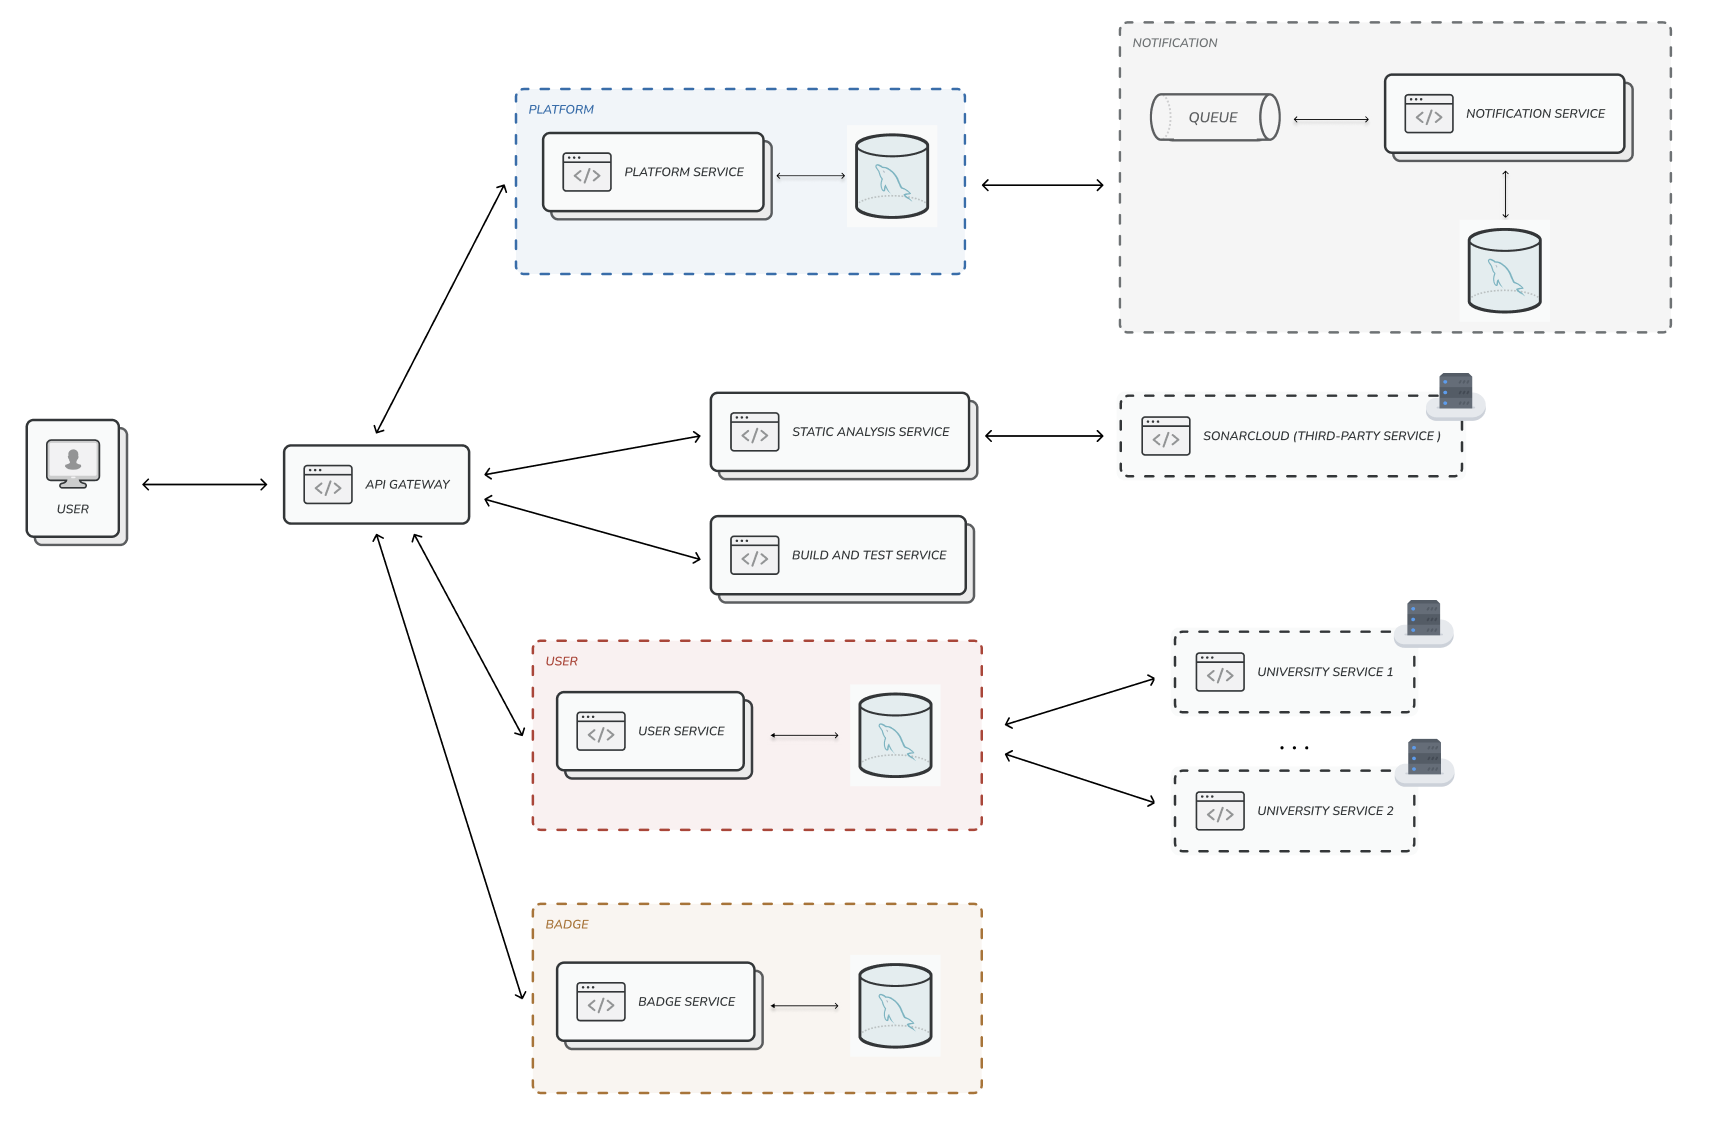
\includegraphics[width=\textwidth]{../images/abstract-system-layout.PNG}
    \caption{Abstract System View}
    \label{fig:Abstract System View}
\end{figure}

These sections contain modules with functionality related to the same domain and independent of each other.
Consequently, the areas will be implemented by different microservices ensuring low coupling and high cohesion.\\
The choice to use microservice architecture allows flexibility and scalability.
All services can indeed be duplicated, since they don't have to interact with databases shared among microservices that could become bottlenecks of the system.\\
In addition, the components involved in sending notifications, compiling sources, running tests, and analyzing them perform more or less complex operations that may take a few moments of execution time.
Consequently, they will be implemented in such a way as to be asynchronous, using of message queues to avoid making users wait for a long time (more details in later sections).


\section{Component view}
\begin{adjustbox}{
        max size={\textwidth}{\textheightwithcaption{1}},
        center,
        caption={Component view diagram},
        label={fig:Component view diagram},
        figure=H}
    \puml{puml/component-view}
\end{adjustbox}

\subsection{Client Components}
The frontend of the platform is a website that allows users to interact with the system.
The role of the website is to interface the user with the API Gateway, rendering interfaces and requesting data.

\subsection{Server Components}
The server components contain the business logic needed to provide the functionalities of the application to the clients,
by responding to requests made by Client Components as well as perform tasks based on interaction with the external
platforms used by the clients (such as GitHub). There are 5 main components, which corresponds to the main areas identified
above, as well as a few additional components:
\begin{itemize}
    \item \textbf{User Service} {-} implements the authentication as well as keeps track of both students and educators by making
          use of 3rd-party authentication services provided by the institutions.
    \item \textbf{Platform Service} {-} implements all the logic related to creating and managing battles and tournaments, including
          calculating the score and keeping track of the leaderboards
    \item \textbf{Badge Service} {-} implements all the logic related to the evaluation and assignment of badges, including the gathering
          of information needed in order to do that (for example Git or GH metadata such as number of commits by students, etc.)
          as well as the actual evaluation of JavaScript code which gets used by educators in order to express the logic of
          specific badges
    \item \textbf{Build and Test Service} {-} implements the Continuous Integration aspect, by building students projects and
          running them against tests for each push
    \item \textbf{Static Analysis Service} {-} abstracts away the interaction with SonarCloud, the 3rd party service which will
          perform the actual static analysis. While SonarCloud already exposes their own API for interaction, it is cumbersome
          (as it requires registering a webhook \cite{SonarCloudWh}, importing the project from the GH slug \cite{SonarCloudGh},
          specifying the required analysis metrics in a quality profile \cite{SonarCloudQp} and waiting for a response on the hook).
          Therefore, by abstracting it away we can use it much more easily and, additionally, make it much less inconvenient to
          replace it should the need arise.
    \item \textbf{Notification Service} {-} responsible for delivering push notifications
          to client devices using external notification APIs (such as the Web Push API \cite{WebPushApi})
    \item \textbf{Website CDN} {-} responsible for serving the static files of the SPA to the clients
    \item \textbf{API Gateway} {-} responsible for connecting together all microservices, it is the component that provides a REST
          interface externally, which the clients will send requests to, which will be implemented by a series of internal calls
          using gRPC \cite{gRPC} to all the other microservices in order to make responses. The component does not implement a specific
          functionality per se, but is in charge of providing an interface to the clients as well as enforcing the correct usage
          of said interface.
\end{itemize}

\subsection{Data Components}
Server Components make use of 4 distinct DBMSes, each with its own schema.
\begin{itemize}
    \item \textbf{User DB} {-} saves data related to the users of the platform. Its ER schema is not shown
          here as it would depend on the 3rd-party service, but it would at least require for each student and
          educator a unique identifier, as well as human-readable identifier to allow users to look up each other
          (so name and surname or an email). Educators and Students are saved in different tables.
          \pagebreak
    \item \textbf{Platform DB}
          \begin{adjustbox}{
                  max size={\textwidth}{\textheightwithcaption{1}},
                  center,
                  caption={Platform ER},
                  label={fig:Platform ER},
                  figure=H}
              \puml{puml/platform-db}
          \end{adjustbox}
          \pagebreak
    \item \textbf{Badge DB}
          \begin{adjustbox}{
                  max size={\textwidth}{\textheightwithcaption{1}},
                  center,
                  caption={Badges ER},
                  label={fig:Badges ER},
                  figure=H}
              \puml{/dd/pulm/components-integration/badge.pulm}
          \end{adjustbox}
    \item \textbf{Notification DB}
          \begin{adjustbox}{
                  max size={\textwidth}{\textheightwithcaption{1}},
                  center,
                  caption={Notification ER},
                  label={fig:Notification ER},
                  figure=H}
              \puml{puml/notification-db}
          \end{adjustbox}
\end{itemize}
\pagebreak

\section{Deployment view}
\begin{adjustbox}{
        max size={\textwidth}{\textheightwithcaption{1}},
        center,
        caption={Deployment view diagram},
        label={fig:Deployment view diagram},
        figure=H}
    \includesvg{images/deployment-diagram.svg}
\end{adjustbox}
The frontend is a SPA implemented with the React framework.
The website can be visited from any modern web browser, such as Google Chrome, Mozilla Firefox or Microsoft Edge.
Clients can be any device that can run the previous browsers, such as computers with Windows, Linux or macOS and smartphones/tablets with Android or IOS.

The website is served by a CDN, such as Cloudflare, Amazon CloudFront or Akamai.
This allows to always have the maximum efficiency, regardless of the number of users connected at the same time.

All other microservices are protected by a firewall that allows only HTTPS connections to the API Gateway.
All microservices can be hosted on-premise or in cloud, within a virtual network, such as Amazon VPC \cite{VPC}.
Since the expected workload will not be constant over time (all students study more or less at the same times),
an on-premise architecture would be unused most of the time, resulting in a waste of money.
The best choice is therefore a cloud architecture, such as Amazon EC2 \cite{EC2}, that allows to scale up resources only when really needed.

The API Gateway is stateless and can be implemented with the Spring Cloud Gateway \cite{SpringCloudGateway}.
It is built on top of the Reactor project \cite{Reactor}, which provides a non-blocking API for routing and filtering requests.
This allows to handle high traffic and scale the API Gateway horizontally when necessary.
The API Gateway is also responsible for performing load balancing in case other microservices are replicated.

If the API Gateway is replicated, a load balancer, such as the Amazon ELB \cite{ELB}, is necessary to equally distribute requests among the various instances.

The Build and Test Service is based on the Jenkins system \cite{Jenkins}.
It is the most CPU-intensive service and should adopt a distributed builds architecture \cite{JenkinsScale}.
One possibility is to have a single Jenkins controller that schedules builds to dedicated build nodes (agents).
Build agents can be dynamically deployed to a new EC2 instance and removed, based on the current workload.\\
If the CKB platform will grow up, an architecture with multiple controllers can be adopted.
For example, the platform can create a Jenkins controller for each tournament.

All other service are implemented as Spring Boot \cite{SpringBoot} applications and they can be deployed to EC2 instances.

The Platform Service, Badge Service, User Service and Notification Service also have their own database.
They use a managed DB service, such as Amazon RDS, that can automatically manage backups and resource scaling.
Each database is in a private subnetwork and it can be accessed only by its corresponding service.

The Notification Service uses RabbitMQ \cite{RabbitMQ} to create a queue where the Platform Service can push messages.
The service will periodically pop messages from the queue with the Spring AMQP project \cite{SpringAMQP} and send them.

\pagebreak

\section{Runtime view}
The following sequence diagrams represent the dynamics of interaction between components.\\
Sequence diagrams from \ref{{RW1}} to \ref{{RW9}} are the realizations of the corresponding use cases in the RASD document.\\
Sequence diagram \ref{{RW0.1}} represents the login process.\\
Sequence diagrams from \ref{{RW0.2}} to \ref{{RW0.5}} are common part that have been extracted for simplicity and are not shown in other diagrams.\\
In the first four sequence diagrams, the user could be a student or an educator.

\begin{enumerate}[label=\textbf{RW\arabic*}:,ref=RW\arabic*,leftmargin=1.3cm]
    \item[]
          \begin{enumerate}[label=\textbf{RW\arabic{enumi}.\arabic*}:,ref=RW\arabic{enumi}.\arabic*,leftmargin=0.5cm]
              \labelledsubitem{
                  \textbf{}
                  \begin{adjustbox}{
                          max size={\textwidth}{\textheightwithcaption{1}},
                          center,
                          caption={Login},
                          label={fig:Login},
                          figure=H}
                      \puml{puml/rw0.1}
                  \end{adjustbox}
                  When the User Service receives the login request, it contacts the external SSO service to validate it.
                  If the credential provided by the user are correct, the User Service returns an authToken, that must be included in all subsequent requests.
                  \pagebreak
              }
              \labelledsubitem{
                  \textbf{}
                  \begin{adjustbox}{
                          max size={\textwidth}{\textheightwithcaption{1}},
                          center,
                          caption={User gets list of tournaments},
                          label={fig:User gets list of tournaments},
                          figure=H}
                      \puml{puml/rw0.2}
                  \end{adjustbox}
              }
              \labelledsubitem{
                  \textbf{}
                  \begin{adjustbox}{
                          max size={\textwidth}{\textheightwithcaption{1}},
                          center,
                          caption={User gets tournament details},
                          label={fig:User gets tournament details},
                          figure=H}
                      \puml{puml/rw0.3}
                  \end{adjustbox}
                  \pagebreak
              }
              \labelledsubitem{
                  \textbf{}
                  \begin{adjustbox}{
                          max size={\textwidth}{\textheightwithcaption{1}},
                          center,
                          caption={User gets battle details},
                          label={fig:User gets battle details},
                          figure=H}
                      \puml{puml/rw0.4}
                  \end{adjustbox}
                  \pagebreak
              }
              \labelledsubitem{
                  \textbf{}
                  \begin{adjustbox}{
                          max size={\textwidth}{\textheightwithcaption{1}},
                          center,
                          caption={Notification is sent},
                          label={fig:Notification is sent},
                          figure=H}
                      \puml{puml/rw0.5}
                  \end{adjustbox}
                  This diagram shows the process of sending a notification.
                  The Notification Service will periodically pop from the Notification Queue messages that contain an array of IDs of the recipient students.
                  Then the Notification Service will look for each student's endpoint URL (previously registered by clients using the API Gateway)
                  and sends the notifications.
                  \pagebreak
              }
          \end{enumerate}

          \labelleditem{
              \textbf{}
              \begin{adjustbox}{
                      max size={\textwidth}{\textheightwithcaption{1}},
                      center,
                      caption={Educator creates a new Tournament},
                      label={fig:Educator creates a new Tournament},
                      figure=H}
                  \puml{puml/rw1}
              \end{adjustbox}
              \pagebreak
          }
          \labelleditem{
              \textbf{}
              \begin{adjustbox}{
                      max size={\textwidth}{\textheightwithcaption{1}},
                      center,
                      caption={Educator creates a new badge},
                      label={fig:Educator creates a new badge},
                      figure=H}
                  \puml{puml/rw2}
              \end{adjustbox}
              \pagebreak
          }
          \labelleditem{
              \textbf{}
              \begin{adjustbox}{
                      max size={\textwidth}{\textheightwithcaption{1}},
                      center,
                      caption={Educator creates a new Battle for an Existing Tournament},
                      label={fig:Educator creates a new Battle for an Existing Tournament},
                      figure=H}
                  \puml{puml/rw3}
              \end{adjustbox}
              \pagebreak
          }
          \labelleditem{
              \textbf{}
              \begin{adjustbox}{
                      max size={\textwidth}{\textheightwithcaption{1}},
                      center,
                      caption={Student joins to an existing Tournament by receiving a notification},
                      label={fig:Student joins to an existing Tournament by receiving a notification},
                      figure=H}
                  \puml{puml/rw4}
              \end{adjustbox}
              \pagebreak
          }
          \labelleditem{
              \textbf{}
              \begin{adjustbox}{
                      max size={\textwidth}{\textheightwithcaption{1}},
                      center,
                      figure=H}
                  \puml{puml/rw5-part1}
              \end{adjustbox}
              \pagebreak
              \begin{adjustbox}{
                      max size={\textwidth}{\textheightwithcaption{1}},
                      center,
                      caption={Students create a team for a tournament battle},
                      label={fig:Students create a team for a tournament battle},
                      figure=H}
                  \puml{puml/rw5-part2}
              \end{adjustbox}
              \pagebreak
          }
          \labelleditem{
              \textbf{}
              \begin{adjustbox}{
                      max size={\textwidth}{\textheightwithcaption{1}},
                      center,
                      caption={Student forks the repository},
                      label={fig:Student forks the repository},
                      figure=H}
                  \puml{puml/rw6}
              \end{adjustbox}
              \pagebreak
          }
          \labelleditem{
              \textbf{}
              \begin{adjustbox}{
                      max size={\textwidth}{\textheightwithcaption{2}},
                      center,
                      caption={Student pushes and triggers automatic evaluation},
                      label={fig:Student pushes and triggers automatic evaluation},
                      figure=H}
                  \puml{puml/rw7}
              \end{adjustbox}
              \pagebreak
          }
          \labelleditem{
              \textbf{}
              \begin{adjustbox}{
                      max size={\textwidth}{\textheightwithcaption{1}},
                      center,
                      caption={Educator manually evaluates teams},
                      label={fig:Educator manually evaluates teams},
                      figure=H}
                  \puml{puml/rw8}
              \end{adjustbox}
              \pagebreak
          }
          \labelleditem{
              \textbf{}
              \begin{adjustbox}{
                      max size={\textwidth}{\textheightwithcaption{1}},
                      center,
                      caption={Educator closes a tournament},
                      label={fig:Educator closes a tournament},
                      figure=H}
                  \puml{puml/rw9}
              \end{adjustbox}
              \pagebreak
          }
\end{enumerate}

\section{Component interfaces}
Here the most relevant interfaces exposed by components are described, including all the operations
seen in the previous diagrams:
\begin{itemize}
    \item \textbf{API Gateway}
          \begin{itemize}
              \item \textbf{login(username: String, password: String): String?}
                    logs the user in through the sso service and, if successful, returns the authToken
              \item \textbf{getListOfTournaments(authToken: String): List<SimpleTournament>}
                    given a valid educator auth token, returns the list of tournaments which he has created
                    or he has permissions to add battles to
              \item \textbf{getTournamentDetails(authToken: String, tournamentId: ID): Tournament}
                    returns the detailed tournament info for the given id
              \item \textbf{getBattleDetails(authToken: String, battleId: ID): Battle}
                    returns the detailed battle info for the given id
              \item \textbf{searchEducator(authToken: String, name: String?, surname: String?, \ldots): ID?}
                    search for an educator matching the given name and/or surname
              \item \textbf{searchStudent(authToken: String, name: String?, surname: String?, \ldots): ID?}
                    search for a student matching the given name and/or surname
              \item \textbf{createTournament(authToken: String, tournamentInfo: NewTournament): ID}
                    create a new tournament with the given info and return its id
              \item \textbf{createBadge(authToken: String, badgeInfo: NewBadge): ID}
                    create a new badge with the given info and return its id
              \item \textbf{createNewBattle(authToken: String, tournementId: ID, battleInfo: Battle): ID}
                    create a new battle with the given info and return its id
              \item \textbf{enrollInTournament(authToken: String, tournementId: ID): void}
                    enroll the student owning the given token in the given tournament
              \item \textbf{createTeam(authToken: String, battleId: ID): ID}
                    create a new team to take part in the given battle and assign the student owning the given token
                    to it, returning the id of the created team
              \item \textbf{invite(authToken: String, newTeamId: ID, invitedStudentId: ID): void}
                    send an invitation for the given team to the invitedStudentId, with the student owning the given token
                    as the invite sender
              \item \textbf{acceptInvitation(authToken: String, invitation: ID): void}
                    accept the given invitation
              \item \textbf{rejectInvitation(authToken: String, invitation: ID): void}
                    reject the given invitation
              \item \textbf{enrollInBattle(authToken: String, teamId: ID): void}
                    enroll the given team in the battle
              \item \textbf{insertRepoSlug(authToken: String, battleId: ID, repo: Slug): void }
                    associate the given GH repository to the team of the student owning the given token for the
                    specified battle
              \item \textbf{newPush(repo: Slug): void }
                    triggered by the GHA on a new push to the specified repository
              \item \textbf{assignGrade(authToken: String, battleId: ID, teamId: ID, grade: Int): void }
                    assign this gradle to the submission of the specified team in the given battle
              \item \textbf{closeTournament(authToken: String, tournamentId: ID): void }
                    close the given tournament
              \item \textbf{closeBattle(authToken: String, battleId: ID): void }
                    close the given battle while it's in its consolidation phase
              \item \textbf{addStudentNotificationEndpoints(authToken: String, endpoint: String): void}
                    add the URL of the notification endpoints of a student
          \end{itemize}
    \item \textbf{User Interface}
          \begin{itemize}
              \item \textbf{login(username: String, password: String): String?}
                    logs the user in through the sso service and, if successful, returns the authToken
              \item \textbf{validateEducatorToken(authToken: String): ID?}
                    validate that the given token is a valid educator token and return its educator id
              \item \textbf{validateStudentToken(authToken: String): ID?}
                    validate that the given token is a valid student token and return its student id
              \item \textbf{searchEducator(name: String?, surname: String?, \ldots): ID?}
                    search for an educator matching the given name and/or surname
              \item \textbf{searchStudent(name: String?, surname: String?, \ldots): ID?}
                    search for a student matching the given name and/or surname
              \item \textbf{checkEducatorIds(educatorsIds: ID[]): Bool}
                    checks that the given ids are all associated to an existing educator
              \item \textbf{checkStudentId(studentId: ID): Bool}
                    checks that the given id is associated to an existing student
          \end{itemize}
    \item \textbf{Platform Interface}
          \begin{itemize}
              \item \textbf{getListOfTournaments(educatorId: ID): List<SimpleTournament>}
                    given an educator id, returns the list of tournaments which he has created
                    or he has permissions to add battles to
              \item \textbf{getTournamentDetails(tournamentId: ID): Tournament}
                    returns the detailed tournament info for the given id
              \item \textbf{getBattleDetails(battleId: ID): Battle}
                    returns the detailed battle info for the given id
              \item \textbf{createTournament(creatorId: ID, tournamentInfo: NewTournament): ID}
                    create a new tournament with the given info and return its id
              \item \textbf{createNewBattle(tournementId: ID, battleInfo: NewBattle): ID}
                    create a new battle with the given info and return its id
              \item \textbf{enrollInTournament(studentId: ID, tournementId: ID): void}
                    enroll the given student in the given tournament
              \item \textbf{createTeam(battleId: ID, studentId: ID): ID}
                    create a new team to take part in the given battle and assign the student owning the given token
                    to it, returning the id of the created team
              \item \textbf{invite(newTeamId: ID, invitedStudentId: ID): void}
                    send an invitation for the given team to the specified student, with the student owning the given token
                    as the invite sender
              \item \textbf{acceptInvitation(invitation: ID): void}
                    accept the given invitation
              \item \textbf{rejectInvitation(invitation: ID): void}
                    reject the given invitation
              \item \textbf{enrollInBattle(teamId: ID): void}
                    enroll the given team in the battle
              \item \textbf{insertRepoSlug(studentId: ID, battleId: ID, repo: Slug): void }
                    associate the given GH repository to the team of the student owning the given token for the
                    specified battle
              \item \textbf{findBattleAndTeamFor(repo: Slug): {battleId: ID, teamId: ID}? }
              \item \textbf{calculateNewScore(battleId: ID, teamId: ID, testsReport: TestReport, stReport: SatReport): void }
              \item \textbf{assignGrade(battleId: ID, teamId: ID, grade: Int): void }
                    assign this gradle to the submission of the specified team in the given battle
              \item \textbf{closeTournament(tournamentId: ID): void }
                    close the given tournament
              \item \textbf{closeBattle(battleId: ID): void }
                    close the given battle while it's in its consolidation phase
          \end{itemize}
    \item \textbf{Badge Interface}
          \begin{itemize}
              \item \textbf{createBadge(creatorId: ID, badgeInfo: NewBadge): ID}
                    create a new badge with the given info and return its id
              \item \textbf{createVariable(name: String, code: String): void}
                    create a new variable that can be used in badges
              \item \textbf{assignBadges(tournament: Tournament): void}
                    evaluate and assign badges to all the students that took part in the given tournament
          \end{itemize}
    \item \textbf{Notification Interface}
          \begin{itemize}
              \item \textbf{addStudentNotificationEndpoints(studentId: ID, endpoint: String): void}
                    add the URL of the notification endpoints of a student
          \end{itemize}
    \item \textbf{Static Analysis Interface}
          \begin{itemize}
              \item \textbf{analyse(repo: Slug): SatReport}
                    run static analysis on the given repository and produce a report
          \end{itemize}
    \item \textbf{Build and Test Interface}
          \begin{itemize}
              \item \textbf{buildAndTest(repo: Slug): TestReport}
                    build the given repository, run its tests and produce a report
          \end{itemize}
\end{itemize}

Types:
\begin{itemize}
    \item \textbf{ID} {-} a unique identifier for a given object, could be a self-incrementing integer or a UUID (depends on the chosen DBMS)
    \item \textbf{Slug} {-} a String identifying a specific GitHub repository, in the format `<username>/<repository>' as can be seen
          in a GitHub project URL
    \item \textbf{SimpleTournament}
          \begin{lstlisting}
{
    id: ID,
    name: String,
    status: Subscribing | InProgress | Closed,
} 
          \end{lstlisting}
    \item \textbf{Tournament}
          \begin{lstlisting}
{
    id: ID,
    name: String,
    status: Subscribing | InProgress | Closed,
    subscriptionDeadline: DateTime,
    enrolledStudents: { id: ID, name: String, score: Int }[],
    battles: { id: ID }[],
} 
          \end{lstlisting}
    \item \textbf{NewTournament}
          \begin{lstlisting}
{
    name: String,
    subscriptionDeadline: DateTime,
    authorizedEducators: { id: ID },
    badges: { id: ID }[],
} 
          \end{lstlisting}
    \item \textbf{Battle}
          \begin{lstlisting}
{
    name: String,
    description: String,
    status: Registration | Submission | Consolidation | Done,
    minStudents: Int,
    maxStudents: Int,
    registrationDeadline: DateTime,
    submissionDeadline: DateTime,
    requiresManualEvaluation: Bool,
    repo: Slug?,
    teams: { id: ID, students: { id: ID }[], score: Int }[],
} 
          \end{lstlisting}
    \item \textbf{NewBattle}
          \begin{lstlisting}
{
    name: String,
    description: String,
    minStudents: Int,
    maxStudents: Int,
    registrationDeadline: DateTime,
    submissionDeadline: DateTime,
    requiresManualEvaluation: Bool,
    zippedProject: Blob,
    privateProjectFiles: Path[],
    sonarRules: {
        key: String,
        parameters: {
            key: String,
            value: String,
        }[],
    }[],
}
          \end{lstlisting}
          The zippedProject field is a binary blob which contains all project files and tests, both public and private.
          The privateProjectFiles is in charge of defining which files from this zip will be hidden from the students,
          so that educators can specify private tests. Care must be taken by educators so that the project build script
          can also work in the absence of those files. The sonarRules field lists all the rules to be applied by
          SonarCloud when scanning.
    \item \textbf{NewBadge}
          \begin{lstlisting}
{
    title: String,
    condition: String,
} 
          \end{lstlisting}
    \item \textbf{TestReport}
          \begin{lstlisting}
{
    passed: Int,
    failed: Int,
} 
          \end{lstlisting}
    \item \textbf{SatReport}
          \begin{lstlisting}
Map<{ metricName: String }, { score: Int }> 
          \end{lstlisting}
\end{itemize}

\section{Selected architectural styles and patterns}
\begin{description}[leftmargin=0pt]
    \item[Fat client:]
          fat clients allow offering a wide variety of functionalities independent from the central server, as well as
          to move part of the business logic off of the server and into the clients.
          The main advantages it offers are greater decoupling of frontend and backend as well as a better interactive
          experience, especially in conditions where the client is on an unstable network.
          Additionally, with the adoption of a single-page applications, there are many cross-platform frameworks
          which allow to reuse code partially or entirely on multiple platforms.
          The single-page web application can also be served by a dedicated static webserver, as all its interactivity is
          implemented client-side, further reducing the burden on the server by delegating its serving to a CDN, which is
          highly optimized for this specific use case.
    \item[REST API:] an architectural style defined on top of HTTP centered around the definition of a standardized
          set of stateless operations. Its main advantages are its simplicity, its use of widely adopted standards which
          facilitate adoption, and its ease of scalability given by its stateless nature. It allows to have a single API
          interface against which a heterogeneous set of clients can make requests.
    \item[Microservices architecture:]
          an architectural style where a single application is developed as a suite of small services,
          each running in its own process and each dealing with a single bounded context in the target domain. The use of
          this architecture allows us a more fine-grained scaling strategy, as we can clearly select in our system CPU-bound
          services (such as the Build and Test Service) which will need to have many more resources allocated to it compared
          to the rest of the system.
    \item[API Gateway:]
          a mediator which sits between clients and a service being invoked, which allows to implement cross-cutting concerns
          such as authentication mechanism common for all microservices. It also makes it possible to keep track of and locate references to the different instances of microservices.
    \item[RPC:] an interaction style where remote calls resembles procedure call in a local setting. In particular, we have
          chosen to use gRPC and adopt its philosophy, centered around ``coarse-grained message exchange while avoiding the
          pitfalls of distributed objects and the fallacies of ignoring the network'' \cite{gRPCPrinciples}, therefore
          avoiding many of the issues normally stemming from RPC/RMI. Additionally, its support out-of-the-box for many
          languages, load-balancing, blocking \& non-blocking support and HTTP transport make it a perfect fit for use in a
          microservice architecture.
    \item[Pub-sub/Message queuing:] a messaging pattern which allows to obtain a high degree of decoupling among components
          in both space and time: a publisher does not need to know of the existence of a subscriber and can continue to
          operate independently even if there is none. By doing so, asynchronous communication is implemented.
    \item[Tiered architecture:] the separation of the architecture in layers, such as presentation, business and data,
          offers great flexibility, maintainability and scalability. In particular, by separating the business from the data
          and having communication between components always go through a predefined API, we do not have to worry about
          each knowing the internal representation of the others.
    \item[Stateless components:] the use of stateless components, which do not have memory of interactions they have previously
          received, allows to decouple successive calls to services and facilitates the horizontal scaling of the system.
\end{description}

\section{Other design decisions}
\begin{description}[leftmargin=0pt]
    \item[Relational DBMS:]
          a relational database is the traditional choice because of their guarantees given by ACID properties
          enforcing consistency on the data, as well as their fixed schema with well-defined entities which fits
          well with the well-defined model we have identified.
\end{description}


\chapter{User Interface Design}
% !TeX root = ../dd.tex

Depending on how communication is implemented between the CKB Platform user service and the university's user management system,
this login screen may allow direct login by interfacing with the university's login or it will simply redirect to the university's login site by subsequently logging in.
\begin{figure}[H]
    \centering
    
\includegraphics[width=\textwidth]{../images/login.png}
    \caption{Login}
    \label{fig:Login}
\end{figure}
\begin{figure}[H]
    \centering
    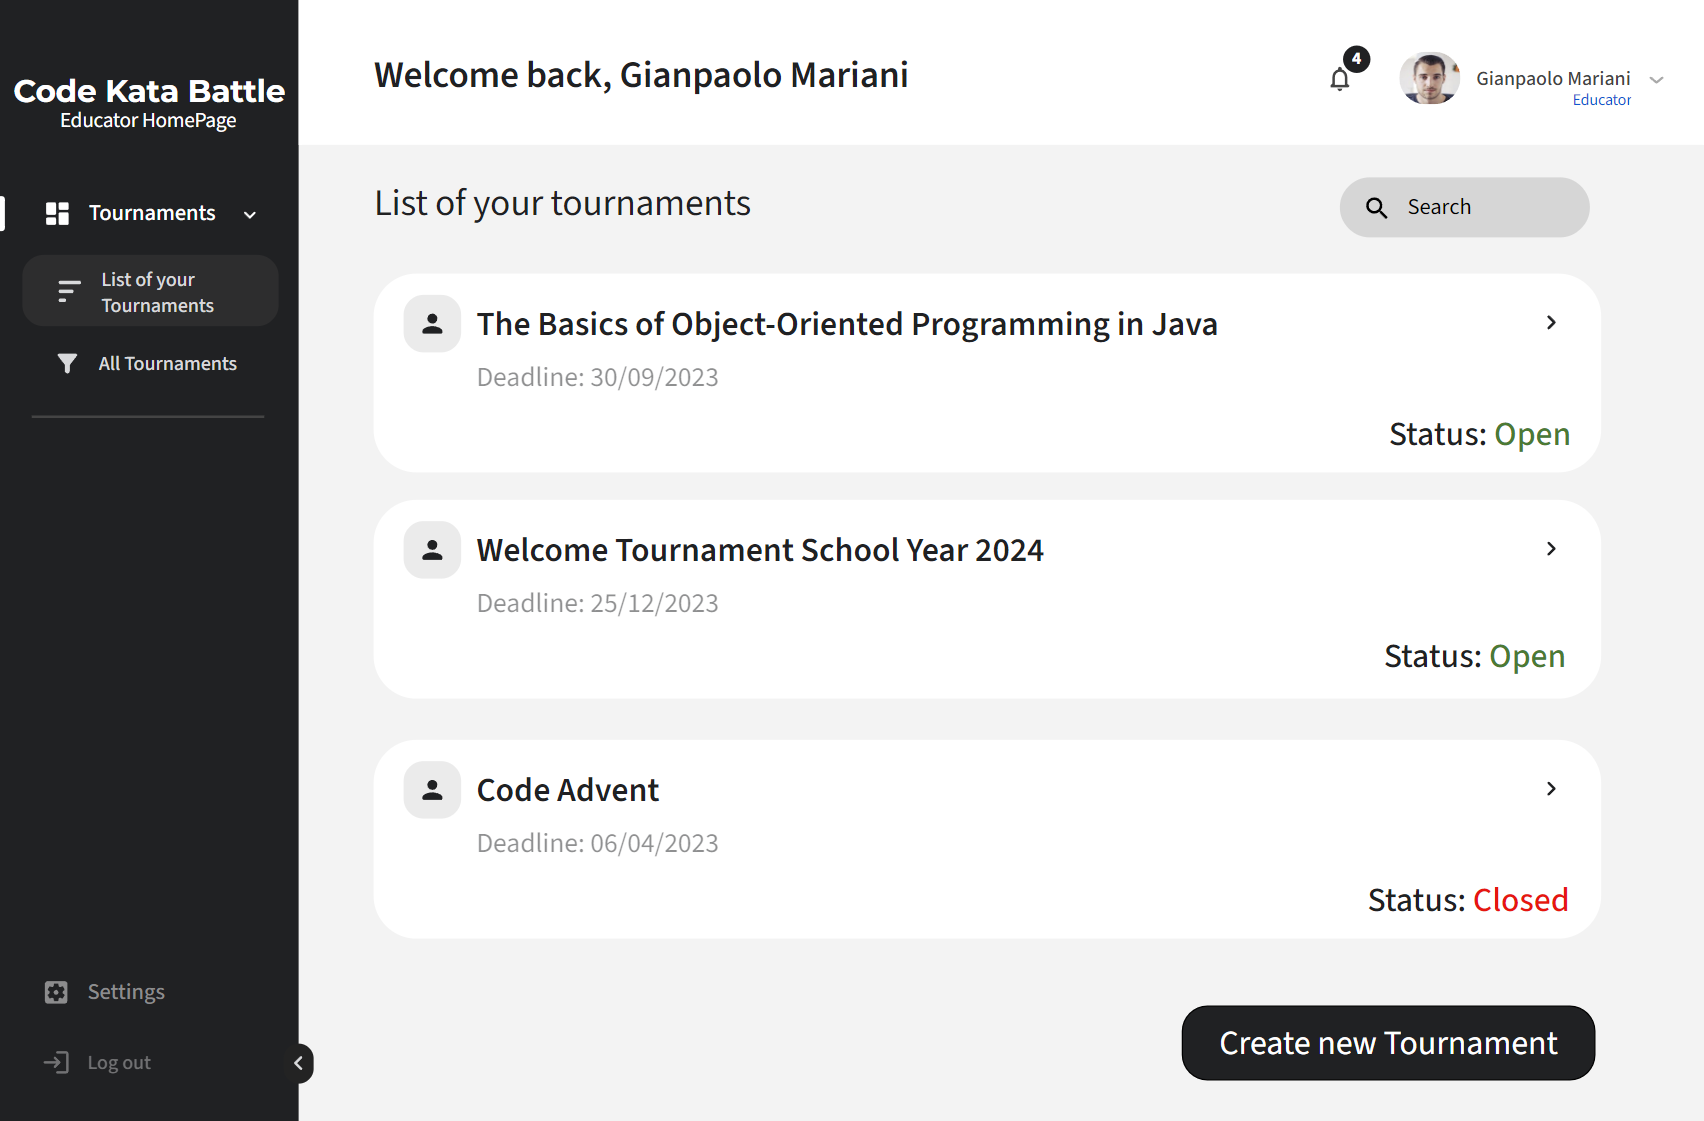
\includegraphics[width=\textwidth]{../images/homepage-educator.png}
    \caption{HomePage Educator}
    \label{fig:HomePage Educator}
\end{figure}
\begin{figure}[H]
    \centering
    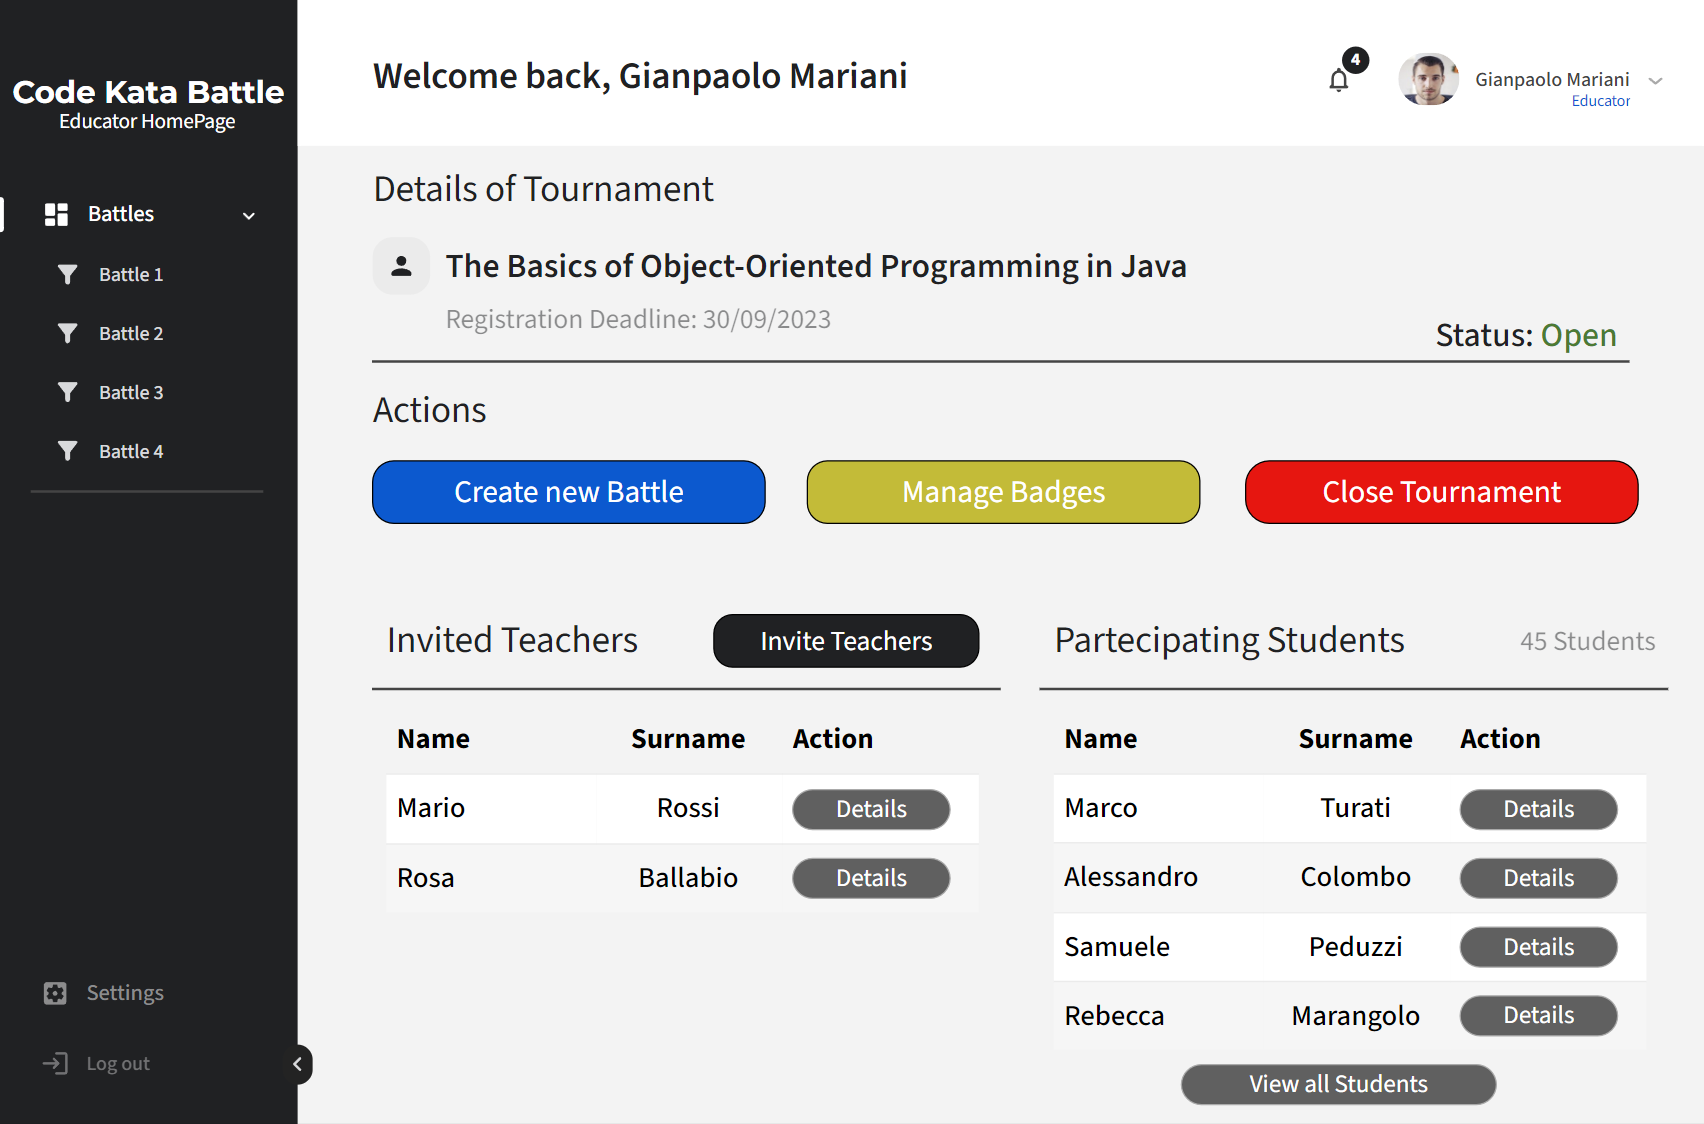
\includegraphics[width=\textwidth]{../images/details-tournament-educator.png}
    \caption{Details Tournament Educator}
    \label{fig:Details Tournament Educator}
\end{figure}
\begin{figure}[H]
    \centering
    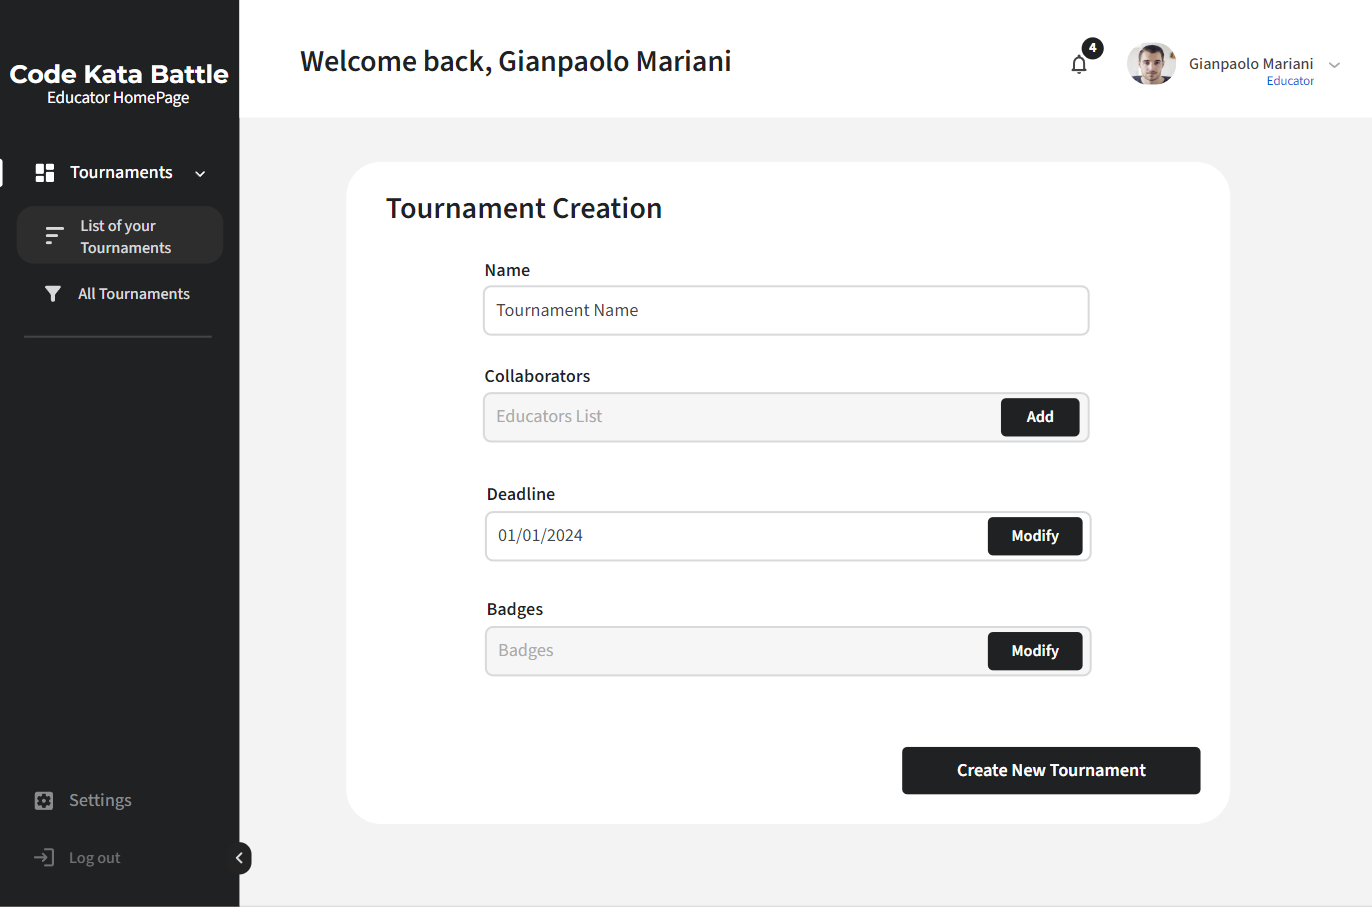
\includegraphics[width=\textwidth]{../images/tournament-creation-educator.png}
    \caption{Details Tournament Educator}
    \label{fig:Details Tournament Educator}
\end{figure}
\begin{figure}[H]
    \centering
    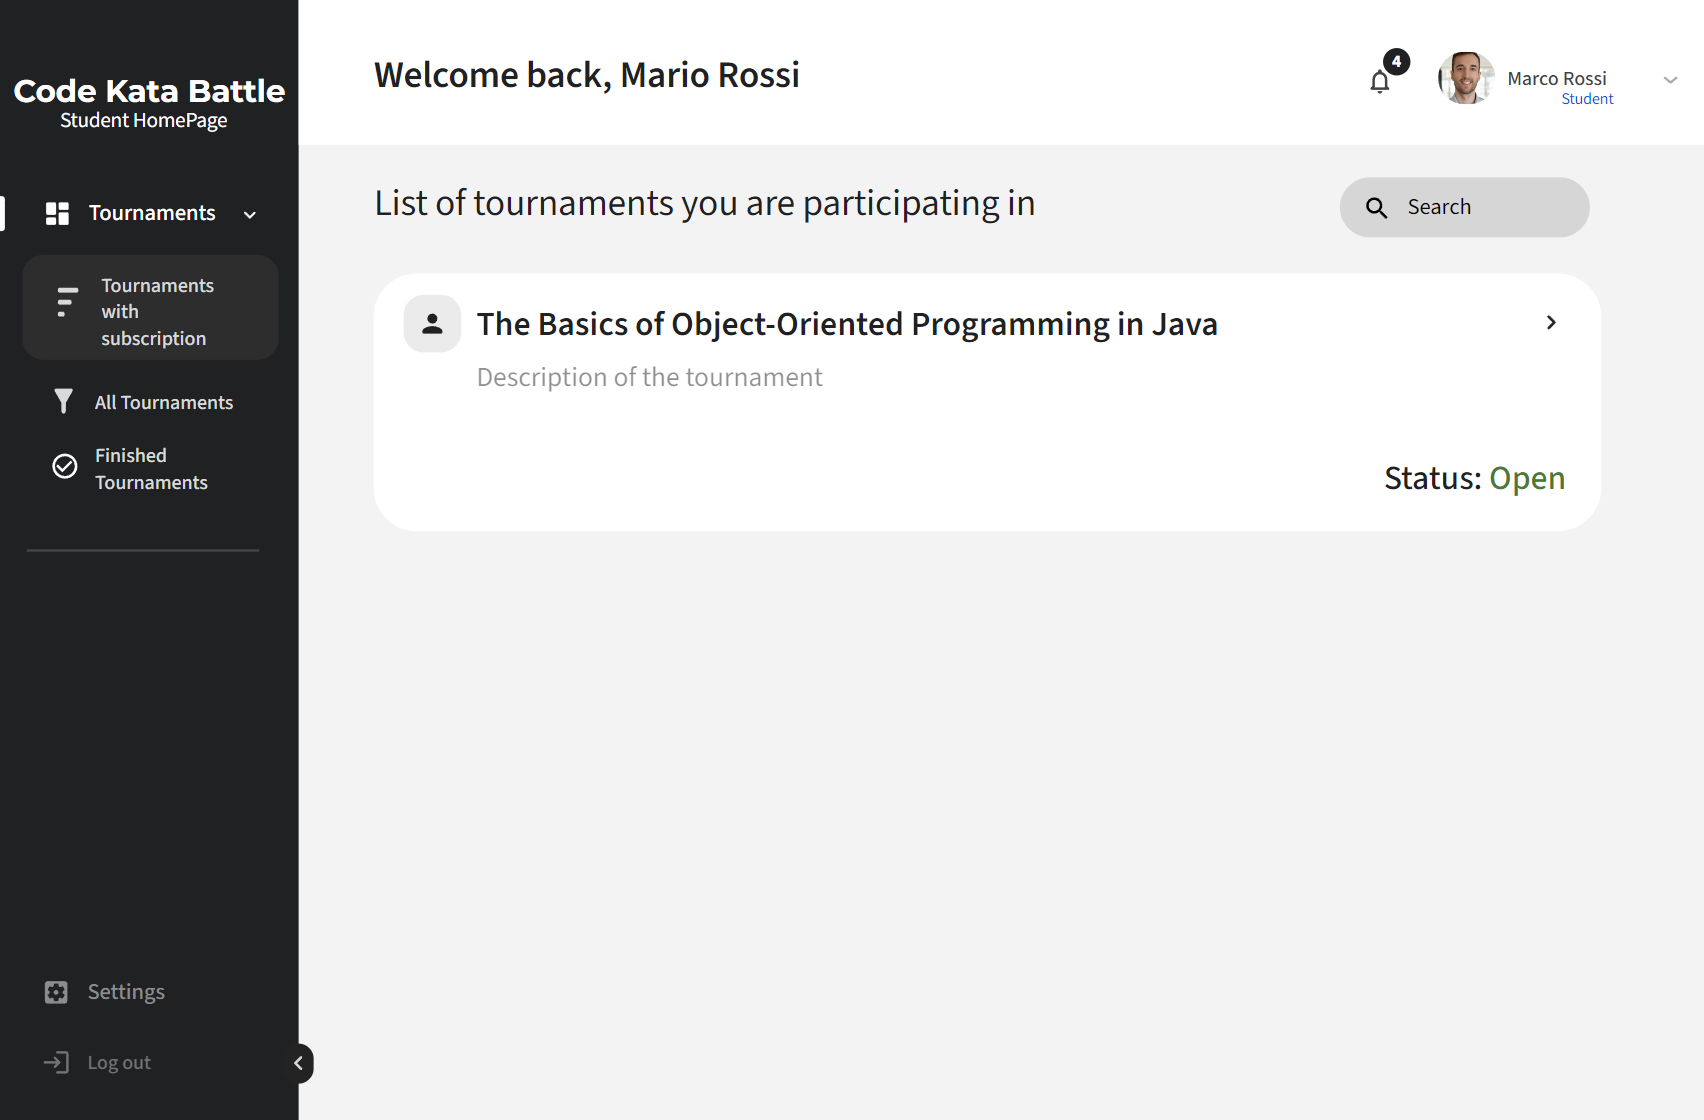
\includegraphics[width=\textwidth]{../images/homepage-student.png}
    \caption{HomePage Student}
    \label{fig:HomePage Student}
\end{figure}
\begin{figure}[H]
    \centering
    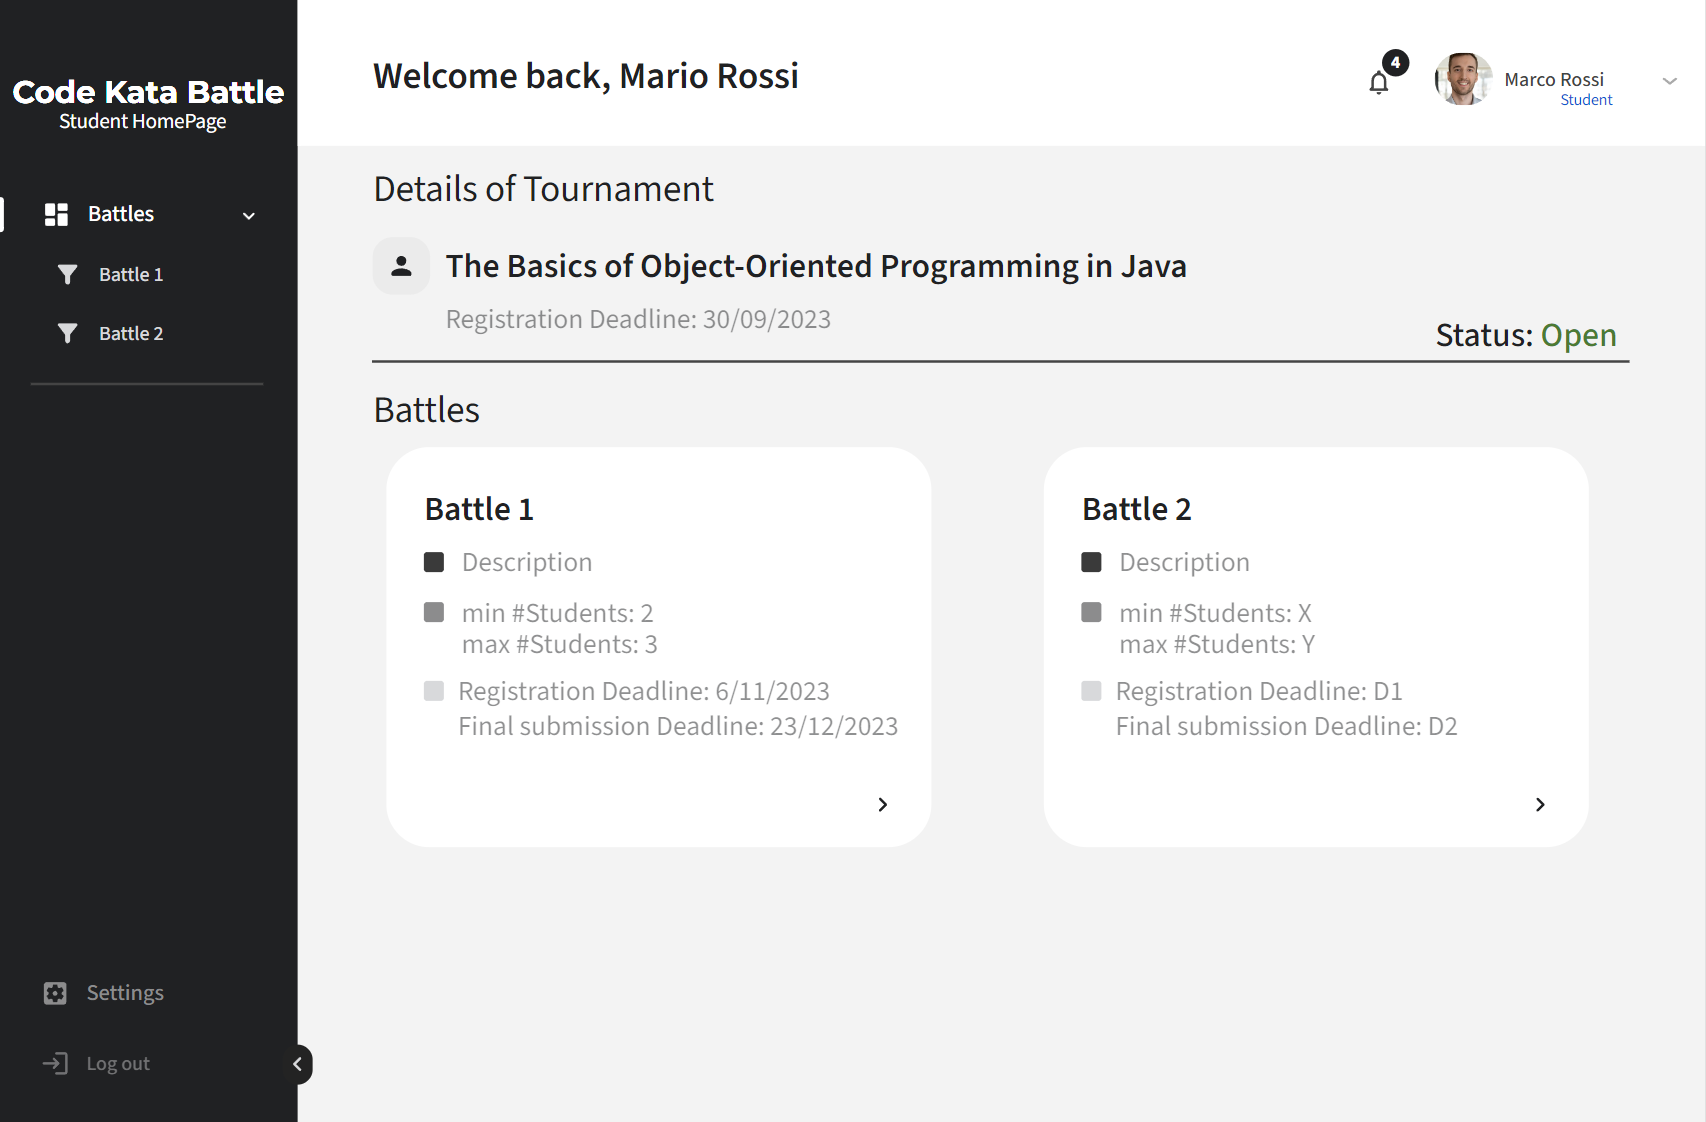
\includegraphics[width=\textwidth]{../images/details-tournament-student.png}
    \caption{Details Tournament Student}
    \label{fig:Details Tournament Student}
\end{figure}




\chapter{Requirements Treceability}
% !TeX root = ../dd.tex
In this section the requirements specified in the RASD are mapped to the components defined above. For brevity,
the API Gateway is omitted as, since it mediates most of the operations, it would need to be specified in almost
all requirements.
\begin{center}
    \begin{longtable}{|l|p{8cm}|p{5cm}|}
        \hline
              & \textbf{Description}                                                                                                                                                           & \textbf{Components}                                                        \\\hline
        \hline
        \endhead
        \hline
        \endfoot
        \hline
        \caption{Components traceability matrix}
        \label{table:Components traceability matrix}
        \endlastfoot
        R1    & The system shall allow users to log in with SSO.                                                                                                                               & \textbf{User Service}                                                      \\\hline
        R2    & The system shall allow the educator to create a tournament.                                                                                                                    & \textbf{Platform Service}                                                  \\\hline
        R2.1  & The system shall allow the educator to specify the subscription deadline of a tournament.                                                                                      & \textbf{Platform Service}                                                  \\\hline
        R2.2  & The system shall allow the educator to grant other colleagues the permission to create battles within the context of a specific tournament.                                    & \textbf{User Service, Platform Service}                                    \\\hline
        R2.3  & The system shall notify the students of the new tournament.                                                                                                                    & \textbf{Platform Service, Notification Service}                            \\\hline
        R2.4  & The system shall allow the educator who create the tournament to close it.                                                                                                     & \textbf{Platform Service}                                                  \\\hline
        R3    & The system shall allow students to subscribe to a tournament.                                                                                                                  & \textbf{Platform Service}                                                  \\\hline
        R4    & The system shall allow the educator to create a battle within the context of a specific tournament.                                                                            & \textbf{Platform Service}                                                  \\\hline
        R4.1  & The system shall allow the educator to set minimum and maximum number of students per group.                                                                                   & \textbf{Platform Service}                                                  \\\hline
        R4.2  & The system shall allow the educator to set a textual description.                                                                                                              & \textbf{Platform Service}                                                  \\\hline
        R4.3  & The system shall allow the educator to set the programming language.                                                                                                           & \textbf{Platform Service}                                                  \\\hline
        R4.4  & The system shall allow the educator to upload a set of test cases.                                                                                                             & \textbf{Platform Service, Build and Test Service}                          \\\hline
        R4.5  & The system shall allow the educator to upload a build automation script.                                                                                                       & \textbf{Platform Service, Build and Test Service}                          \\\hline
        R4.6  & The system shall allow the educator to set a registration deadline.                                                                                                            & \textbf{Platform Service}                                                  \\\hline
        R4.7  & The system shall allow the educator to set a final submission deadline.                                                                                                        & \textbf{Platform Service}                                                  \\\hline
        R4.8  & The system shall allow the educator to enable manual evaluation.                                                                                                               & \textbf{Platform Service}                                                  \\\hline
        R4.9  & The system shall allow the educator to select aspects that should be evaluated by the static analysis tool, such as security, reliability, and maintainability.                & \textbf{Platform Service, Static Analysis Service}                         \\\hline
        R4.10 & The system shall notify students subscribed to a tournament of the creation of a new battle.                                                                                   & \textbf{Platform Service, Notification Service}                            \\\hline
        R5    & The system shall allow students to join a battle, respecting the minimum and maximum number of students per group.                                                             & \textbf{Platform Service}                                                  \\\hline
        R5.1  & The system shall allow students to invite other students to join a battle.                                                                                                     & \textbf{Platform Service, User Service}                                    \\\hline
        R5.2  & The system shall allow students to accept received invitation.                                                                                                                 & \textbf{Platform Service}                                                  \\\hline
        R6    & When the registration deadline expires, the system shall create a GitHub repository containing the code kata.                                                                  & \textbf{Platform Service}                                                  \\\hline
        R7    & The system shall send the link to all students who are members of subscribed teams.                                                                                            & \textbf{Notification Service}                                              \\\hline
        R8    & The system shall expose an API that can by called by the GitHub Action platform.                                                                                               & \textbf{API Gateway}                                                       \\\hline
        R9    & On each push, the system shall calculate and update the battle score of the team.                                                                                              & \textbf{Platform Service, Build and Test Service, Static Analysis Service} \\\hline
        R9.1  & The system shall pull the latest sources.                                                                                                                                      & \textbf{Build and Test Service}                                            \\\hline
        R9.2  & The system shall analyze quality level of the sources, based on the aspect selected by the educator.                                                                           & \textbf{Static Analysis Service}                                           \\\hline
        R9.3  & The system shall run tests uploaded by the educator.                                                                                                                           & \textbf{Build and Test Service}                                            \\\hline
        R9.4  & The system shall measure the time passed between the registration deadline and the last commit.                                                                                & \textbf{Platform Service}                                                  \\\hline
        R10   & The system shall allow students and educators involved in the battle to see the current rank evolving during the battle.                                                       & \textbf{Platform Service}                                                  \\\hline
        R11   & When the submission deadline expires, if manual evaluation is required, the system shall change the state of the battle to the consolidation stage.                            & \textbf{Platform Service}                                                  \\\hline
        R12   & When the submission deadline expires, if manual evaluation is not required, the system shall close the battle.                                                                 & \textbf{Platform Service}                                                  \\\hline
        R13   & During the consolidation stage, if manual evaluation is required, the system shall allow the educator to go through the sources produced by each team to assign his/her score. & \textbf{Platform Service}                                                  \\\hline
        R14   & At the end of a battle, the system shall calculate the final rank.                                                                                                             & \textbf{Platform Service}                                                  \\\hline
        R15   & When the final rank is available, the system shall notify all students participating in the battle.                                                                            & \textbf{Platform Service, Notification Service}                            \\\hline
        R16   & At the end of each battle, the platform updates the personal tournament score of each student, that is the sum of all battle scores received in that tournament.               & \textbf{Platform Service}                                                  \\\hline
        R17   & The system shall allow users to see the tournament ranks.                                                                                                                      & \textbf{Platform Service}                                                  \\\hline
        R18   & At the end of a tournament, the system shall calculate the final tournament rank.                                                                                              & \textbf{Platform Service}                                                  \\\hline
        R19   & When the final tournament rank is available, the system shall notify all students involved in the tournament.                                                                  & \textbf{Platform Service, Notification Service}                            \\\hline
        R20   & The system shall allow the educator who create a tournament, to create badges within the context of the tournament.                                                            & \textbf{Platform Service, Badge Service}                                   \\\hline
        R20.1 & The system shall allow the educator to specify the title of the badge.                                                                                                         & \textbf{Badge Service}                                                     \\\hline
        R20.2 & The system shall allow the educator to create a new variable that represent any piece of information available in the platform relevant for scoring.                           & \textbf{Badge Service}                                                     \\\hline
        R20.3 & The system shall allow the educator to specify one or more rules that must be fulfilled to achieve the badge, based on variables.                                              & \textbf{Badge Service}                                                     \\\hline
        R20.4 & The system shall allow users to visualize badges collected by a student.                                                                                                       & \textbf{Badge Service}                                                     \\\hline
        R21   & At the end of a tournament, the system shall assign badges to the student who fulfilled the rules.                                                                             & \textbf{Badge Service}                                                     \\\hline
    \end{longtable}
\end{center}


\chapter{Implementation, Integration and Test Plan}
% !TeX root = ../dd.tex

The chosen architecture guarantees high decoupling between components, so that most of them
can be developed and unit tested completely independently, without the need to mock other
components. Once those are developed, we can integrate them at the end and do additional
integration testing. We can identify a few different types components:

\begin{description}[leftmargin=0pt]
    \item[Independent components:] these are back-end components that can be developed fully independently
          from one another and do not need to directly integrate with any other service
    \item[External components:] these are the components provided by third-parties, which are supposed
          to be already reliable, but may need to be stubbed when unit testing our own services
    \item[Integrating components:] these are the back-end components whose sole role is of allowing
          communication between other services and therefore need to be directly integrated with those
    \item[Front-end components:] these are the presentational components that belong to the client layer
          which rely on the back-end REST API, they can therefore be unit tested by mocking it
\end{description}

In order to visualize how much each component will need to be tested and plan accordingly, we can use
the following table, where we associate to each piece of functionality the difficulty of its
implementation and its importance for the final user experience:

\begin{table}[H]
    %\caption*{\textbf{Title}}
    \centering
    \begin{tabular}{|l|l|l|}
        \hline
        \textbf{Feature}                    & \textbf{Importance} & \textbf{Difficulty} \\\hline
        Login                               & High                & Medium              \\
        Tournament and Battle Management    & High                & Low                 \\
        Tournament and Battle Participation & High                & Medium              \\
        Automatic evaluation                & High                & High                \\
        Manual evaluation                   & High                & Low                 \\
        Tournament rankings                 & Medium              & Low                 \\
        Battle rankings                     & Medium              & Low                 \\
        Notifications                       & Medium              & High                \\
        Badges Management                   & Low                 & Medium              \\
        Badges Assignment                   & Low                 & High                \\
        Badges Visualization                & Low                 & High                \\\hline
    \end{tabular}
    \caption{Importance and difficulty of features}
    \label{table:Importance and difficulty of features}
\end{table}

\section{Development and Test Plan}
All the components will be developed and tested using a bottom-up approach, in order to reduce as
much as possible stubs and mocks, which would add additional overhead to the development.
All the independent microservices can be developed first and in parallel, prioritizing components
of high importance which need to be tested more thoroughly as outlined by the table above.
Development can also start on front-end components, which can mock the REST API during testing.
Lastly, integrating components such as the API Gateway can be developed, after which everything
can be integration tested. 

After that is completed, system and e2e testing should be done to verify the adherence to the specified requirements.
This phase also include:
\begin{itemize}
    \item Performance testing, to detect bottlenecks and test the scaling strategies. 
    \item Load testing, to identify memory leaks, overflows and other memory-related problems.
    \item Stress testing: to make sure that the system recovers gracefully after failures.
\end{itemize}
Once a beta version of the software is available, it's possible to perform some acceptance testing which should
involve different users, including stakeholders, to test if the system responds to actual needs and constraints.
\pagebreak
\section{Components integration}
Here components and subsystems are illustrated via graphs. \\
Subsystems are a group of components meant to be integration tested together after unit testing.\\
Integration testing is carried out in a bottom-up approach, so drivers must be implemented to test the different independent subsystems as each subsystem is developed.\\
The first components that can be tested together are the Notification Service and RabbitMQ.
That's because the subsystem is implementing medium importance features and thus proper testing with the queue needs to be done carefully.
\begin{adjustbox}{
        max size={\textwidth}{\textheightwithcaption{1}},
        center,
        caption={Notitification subsystem},
        label={fig:Notitification subsystem},
        figure=H}
    \puml{puml/components-integration/notification}
\end{adjustbox}

Then the Platform subsystem can be integreted with the Queue of the Notification subsystem.
Obtaining the Platform and Notification Subsystem.
\begin{adjustbox}{
        max size={\textwidth}{\textheightwithcaption{1}},
        center,
        caption={Platform and Notification subsystem},
        label={fig:Platform and Notification subsystem},
        figure=H}
    \puml{puml/components-integration/platform-queue}
\end{adjustbox}

The following four subsystems might be developed in any order, or simultaneously, as they do not depend
on each other.
It is recommended to develop first the subsystems that implement High Importance features, such as:\\
the User subsystem, the Build and Test subsystem, and the Static Analysis subsystem, and then the Badge subsystem that implements Low Importance functionality.
\begin{adjustbox}{
        max size={\textwidth}{\textheightwithcaption{1}},
        center,
        caption={User subsystem},
        label={fig:User subsystem},
        figure=H}
    \puml{puml/components-integration/user}
\end{adjustbox}

\begin{adjustbox}{
        max size={\textwidth}{\textheightwithcaption{1}},
        center,
        caption={Build and Test subsystem},
        label={fig:Build and Test subsystem},
        figure=H}
    \puml{puml/components-integration/buildtest}
\end{adjustbox}

\begin{adjustbox}{
        max size={\textwidth}{\textheightwithcaption{1}},
        center,
        caption={Static Analysis subsystem},
        label={fig:Static Analysis  subsystem},
        figure=H}
    \puml{puml/components-integration/staticanalysis}
\end{adjustbox}

\begin{adjustbox}{
        max size={\textwidth}{\textheightwithcaption{1}},
        center,
        caption={Badge subsystem},
        label={fig:Badge subsystem},
        figure=H}
    \puml{puml/components-integration/badge}
\end{adjustbox}

After that we can also develop the Website CDN.
\begin{adjustbox}{
        max size={\textwidth}{\textheightwithcaption{1}},
        center,
        caption={Website CDN subsystem},
        label={fig:Website CDN subsystem},
        figure=H}
    \puml{puml/components-integration/website}
\end{adjustbox}

At this point all subsystems have been implemented and tested, so the next step is performing integration
testing between the subsystems and the API Gateway.
\begin{adjustbox}{
        max size={\textwidth}{\textheightwithcaption{1}},
        center,
        caption={API Gateway subsystem},
        label={fig:API Gateway subsystem},
        figure=H}
    \puml{puml/components-integration/apigateway}
\end{adjustbox}

The integration of all the different subsystems with the Gateway API is a critical operation and performing it all at once will likely lead to errors (because of the big-bang like approach).
To avoid this, the integration can be broken down into smaller integrations by continuing to follow the bottom-up approach.\\
We can proceed to integrate the API Gateway with the Platform and Notification subsystem.

\begin{adjustbox}{
        max size={\textwidth}{\textheightwithcaption{1}},
        center,
        caption={API Gateway subsystem step 1},
        label={fig:API Gateway subsystem step 1},
        figure=H}
    \puml{puml/components-integration/api-integration1}
\end{adjustbox}

Then, it's possible to integrate the API Gateway with the User and the Badge subsystems.


\begin{adjustbox}{
        max size={\textwidth}{\textheightwithcaption{1}},
        center,
        caption={API Gateway subsystem step 2},
        label={fig:API Gateway subsystem step 2},
        figure=H}
    \puml{puml/components-integration/api-integration2}
\end{adjustbox}

After that, integrate the API Gateway with the Static Analysis and Build and Test subsystems.

\begin{adjustbox}{
        max size={\textwidth}{\textheightwithcaption{1}},
        center,
        caption={API Gateway subsystem step 3},
        label={fig:API Gateway subsystem step 3},
        figure=H}
    \puml{puml/components-integration/api-integration3}
\end{adjustbox}

Finally, when all is integrated and tested successfully we can proceed to integrate it with the Website CDN.

\begin{adjustbox}{
        max size={\textwidth}{\textheightwithcaption{1}},
        center,
        caption={API Gateway subsystem step 4},
        label={fig:API Gateway subsystem step 4},
        figure=H}
    \puml{puml/components-integration/api-integration4}
\end{adjustbox}

\chapter{Effort Spent}
% !TeX root = ../rasd.tex
\begin{table}[H]
      %\caption*{\textbf{Title}}
      \centering
      \begin{tabular}{|l|l|l|}
            \hline
            \textbf{Member of group }                  & \textbf{Chapter}            & \textbf{Time spent} \\\hline
            \multirow{4}{*}{\textbf{Mattia Brianti}} & Introduction                & 8h                  \\
                                                       & Overall Description         & 0h                \\
                                                       & Specific Requirements       & 0h                 \\
                                                       & Formal analysis using alloy & 5h                 \\\hline
            \multirow{4}{*}{\textbf{Alex Hathaway}} & Introduction                & 0h                  \\
                                                       & Overall Description         & 0h                  \\
                                                       & Specific Requirements       & 0h                  \\
                                                       & Formal analysis using alloy & 0h                  \\\hline
            \multirow{4}{*}{\textbf{Mattia Rainieri}} & Introduction                & 0h                  \\
                                                       & Overall Description         & 0h                 \\
                                                       & Specific Requirements       & 0h                  \\
                                                       & Formal analysis using alloy & 0h                \\\hline
      \end{tabular}
      \caption{Time spent by each member of group.}
      \label{table:Time spent}
\end{table}


%-------------------------------------------------------------------------
%	BIBLIOGRAPHY
%-------------------------------------------------------------------------

\addtocontents{toc}{\vspace{2em}} % Add a gap in the Contents, for aesthetics
\nocite{*}
\bibliography{bibliography} % The references information are stored in the file named "Thesis_bibliography.bib"


% LIST OF FIGURES
\listoffigures
% LIST OF TABLES
\listoftables

\cleardoublepage

\end{document}
